%%
% Plantilla de Memoria
% Modificación de una plantilla de Latex de Nicolas Diaz para adaptarla 
% al castellano y a las necesidades de escribir informática y matemáticas.
%
% Editada por: Mario Román
%
% License:
% CC BY-NC-SA 3.0 (http://creativecommons.org/licenses/by-nc-sa/3.0/)
%%

%%%%%%%%%%%%%%%%%%%%%
% Thin Sectioned Essay
% LaTeX Template
% Version 1.0 (3/8/13)
%
% This template has been downloaded from:
% http://www.LaTeXTemplates.com
%
% Original Author:
% Nicolas Diaz (nsdiaz@uc.cl) with extensive modifications by:
% Vel (vel@latextemplates.com)
%
% License:
% CC BY-NC-SA 3.0 (http://creativecommons.org/licenses/by-nc-sa/3.0/)
%
%%%%%%%%%%%%%%%%%%%%%

%----------------------------------------------------------------------------------------
%	PAQUETES Y CONFIGURACIÓN DEL DOCUMENTO
%----------------------------------------------------------------------------------------

%% Configuración del papel.
% microtype: Tipografía.
% mathpazo: Usa la fuente Palatino.
\documentclass[a4paper, 10pt]{article}
\usepackage[protrusion=true,expansion=true]{microtype}
\usepackage{mathpazo}

% Requisitos de formato pedidos por el profesor:
\renewcommand{\rmdefault}{phv} % Arial
\renewcommand{\sfdefault}{phv} % Arial
\usepackage[top=2.5cm, bottom=2.5cm, left=3cm, right=3cm]{geometry} % Márgenes

% Hipervínculos
\usepackage[hidelinks]{hyperref}

% Títulos de las figuras
\usepackage[font=large,labelfont=bf]{caption}

% Indentación de párrafos para Palatino
\setlength{\parindent}{0pt}
  \parskip=8pt
\linespread{1.05} % Change line spacing here, Palatino benefits from a slight increase by default


%% Castellano.
% noquoting: Permite uso de comillas no españolas.
% lcroman: Permite la enumeración con numerales romanos en minúscula.
% fontenc: Usa la fuente completa para que pueda copiarse correctamente del pdf.
\usepackage[spanish,es-noquoting,es-lcroman]{babel}
\usepackage[utf8]{inputenc}
\usepackage[T1]{fontenc}
\selectlanguage{spanish}


%% Gráficos
\usepackage{graphicx} % Required for including pictures
\usepackage{wrapfig} % Allows in-line images
\usepackage[usenames,dvipsnames]{color} % Coloring code


%% Matemáticas
\usepackage{amsmath}


%% Bibliografía
\makeatletter
\renewcommand\@biblabel[1]{\textbf{#1.}} % Change the square brackets for each bibliography item from '[1]' to '1.'
\renewcommand{\@listI}{\itemsep=0pt} % Reduce the space between items in the itemize and enumerate environments and the bibliography



%----------------------------------------------------------------------------------------
%	TÍTULO
%----------------------------------------------------------------------------------------
% Configuraciones para el título.
% El título no debe editarse aquí.
\renewcommand{\maketitle}{
  \begin{flushright} % Right align
  
  {\LARGE\@title} % Increase the font size of the title
  
  \vspace{50pt} % Some vertical space between the title and author name
  
  {\large\@author} % Author name
  \\\@date % Date
  \vspace{40pt} % Some vertical space between the author block and abstract
  \end{flushright}
}

% Título
\title{\textbf{Ingeniería de Servidores}\\ % Title
Análisis comparativo de Tomcat, WildFly y GlassFish} % Subtitle

		%Comentado ya que se supone que es anónimo
\author{ %\textsc{Óscar Bermúdez Garrido} % Author
%\\
{\textit{Universidad de Granada}}} % Institution

\date{\today} % Date



%----------------------------------------------------------------------------------------
%	DOCUMENTO
%----------------------------------------------------------------------------------------

\begin{document}

\maketitle % Print the title section

% Resumen (Descomentar para usarlo)
\renewcommand{\abstractname}{Resumen} % Uncomment to change the name of the abstract to something else
\begin{abstract}
	 En este documento, realizaremos un análisis comparativo de tres aplicaciones
	 de software libre, multiplataforma y escritas en Java utilizadas comúnmente
	 como base de servidores webs aunque no son exclusivos de éstos.
	 
	 Para ello, previamente aprenderemos una serie de conceptos básicos para el
	 entendimiento del resto del documento, por ejemplo, J2EE.
	 
	 Después, veremos una pequeña descripción de los 3 programas que compararemos
	 más adelante, así como una pequeña guía de inicio de servicio para cada uno
	 de ellos:
	 
	 \begin{itemize}
	 	\item El contenerdor de servlets y JSP's Apache Tomcat(y su extensión a 
	 	servidor de aplicaciones Apache TomEE).
	 	\item El servidor de aplicaciones WildFly.
	 	\item El servidor de aplicaciones GlassFish.
	 \end{itemize}
	 
	 Una vez presentados e instalados los programas, toca planear el experimento,
	 exponerlo, realizarlo, mostrar los resultados e interpretarlos.
	 
	 Para finalizar, se proponen una serie de posibles estudios que se pueden
	 realizar en el mismo campo de estudio de este documento.
\end{abstract}

% Índice (Descomentar para usarlo)
%{\parskip=2pt
%  \tableofcontents
%}
%\pagebreak

%% Inicio del documento

\section{Introducción}
	La sociedad de nuestros días se caracteriza por la obtención, almacenamiento y
	utilización de la información. Esta información se utiliza de múltiples maneras,
	desde búsquedas personalizadas en ciertos buscadores webs hasta su uso por parte
	de las empresas publicitarias para mejorar sus técnicas de Marketing.
	
	Por tanto, los sistemas encargados del tratamiento de dicha información causan
	gran impacto en nuestra sociedad. Por la importancia que se le da a la información
	tratada, estos sistemas se desarrollan de forma muy rápida y, de forma análoga a
	ellos, también sus necesidades de capacidades hardware para su correcto funcionamiento.
	
	Esto se traduce en una necesidad de desarrollo forzado de las plataformas que dan
	soporte a dichas tecnologías. Y este desarrollo, a su vez, ocasiona problemas que,
	al solucionarlos, dan lugar a nuevas tecnologías. Uno de estos problemas sería el de
	la comunicación entre sistemas diferentes, ya sea por su sistema operativo, sus
	capacidades hardware o su adaptabilidad y tolerancia a errores.
	
	Una de las posibles soluciones a dicho problema(pero no la única) es la utilización
	de servicios webs. Quizás la mayor ventaja de la utilización de servidores web como
	solución a dicho problema es la posibilidad de interacción entre aplicaciones
	implementadas en diferentes sistemas operativos(o el mismo), esto es, la
	interoperatibilidad, que es aprovechada por los sistemas distribuidos.
	
	Para favorecer dicha interoperabilidad, se fomenta el desarrollo de estándares y
	protocolos que definan cómo deben comunicarse los procesos para obtener una
	colaboración satisfactoria y simplificada, permitiendo así maximizar la eficiencia
	del servicio.
	
	En el desarrollo de servidores webs, se requieren una serie de instrucciones de
	administración de servidores como puede ser control de seguridad, manejo de
	transacciones, escabilidad, concurrencia, gestión de complementos desplegados,
	gestión de peticiones de clientes,\dots que no siempre son fáciles de gestionar por
	el desarrollador. Aunque el desarrollador sea capaz de administrar adecuadamente el
	servidor web, éste esfuerzo adicional distrae la atención sobre la lógica de negocio,
	que debería ser el centro de desarrollo de nuestro servidor web.
	
	Para facilitar el desarrollo de los servidores webs, se desarrollaron plataformas y
	protocolos que se encargan de dichas labores de mantenimiento de bajo nivel permitiendo
	centrar las preocupaciones del desarrollador en la lógica de negocio. Ejemplos de estas
	plataformas serían las plataformas J2EE, Appaserver, .NET, GNUstepWeb, Happstack y
	Django-cms.
	
	Todas estas alternativas se basan en el desarrollo de clientes y servicios webs. En
	este documento, nos centraremos en la plataforma J2EE aunque también se podría exponer
	gran variedad de servidores de aplicaciones basados en cualquiera de las otras plataformas.
	
	Dentro de la plataforma J2EE, podemos encontrar un gran abanico de posibilidades distintas
	para escoger. Entre ellas, destacan Apache Geronimo, Apache TomEE, GlassFish, WildFly
	(anteriormente conocido como JBoss), WebSphere AS, WebLogic Server y JOnAS application
	server.
	
	Al ser opciones tan heterogéneas, ocasiona grandes dudas sobre cuál se habitúa mejor a
	nuestras necesidades, que se ven amplificadas por la mitificación de las propiedades
	que dichas aplicaciones poseen.
	
	En este proyecto, se tratarán de conocer los puntos fuertes y puntos débiles de algunas
	de las plataformas anteriormente citadas. En concreto, se hará sobre Apache Tomcat(aunque
	éste no es un servidor de aplicaciones propiamente dicho como los otros, si no más bien
	es sólo un contenedor de servlets y JSP's), WildFly y GlassFish.
	
	Todos ellos son proyectos de software libre implementados en Java que siguen los
	estándares definidos por la plataforma J2EE y son multiplataforma.
	
\section{Definiciones previas}
	Antes de comenzar, conviene dejar claros algunos conceptos importantes que irán
	apareciendo	a lo largo del documento\footnote{Aunque no lo indique explícitamente,
	estas definiciones son copia, traducción y/o resumen de la página que doy como
	referencia.}:

	\begin{itemize}
		\item \textbf{J2EE}(también conocido como \textit{Java Platform, Enterprise
		Edition} o \textit{Java EE}): es una plataforma de programación de desarrollo y
		ejecución de aplicaciones Java. Para facilitar dicho desarrollo, dispone de una
		serie de API's(RMI, JMS,\dots) así como servlets y JavaService Pages que se encargan
		de las tareas de mantenimiento de bajo nivel(seguridad, escalabilidad,
		concurrencia,\dots) permitiendo al desarrollador centrarse en la lógica de negocio.\cite{J2EE_Def}
		
		\item \textbf{API}(\textit{Application Programming Interface}): Conjunto de rutinas,
		protocolos y herramientas para facilitar el desarrollo de aplicaciones software.
		Ejemplos de API's serían los estándar POSIX o la STL de C++.\cite{API_Def}
		
		\item \textbf{RMI}(\textit{Remote Method Invocation}): API de Java que permite la
		llamada a métodos de forma remota, lo que permite la comunicación entre servidores
		basados en Java.\cite{RMI_Def}
		
		\item \textbf{JMS}(\textit{Java Message Service}): API de Java que permite el envío
		y la recepción de mensajes entre clientes.\cite{JMS_Def} Puede ser:
		\begin{itemize}
			\item Punto a Punto: un cliente le envía un mensaje a otro.
			\item Publicar/Suscribir: un cliente envía el mensaje y varios lo reciben.
		\end{itemize}

		\item \textbf{Servlet}: Programa implementado en Java que se ejecuta en un servidor
		(usualmente en un servidor web) y que responde a las peticiones de los clientes,
		extendiendo así las capacidades del servidor.\cite{Servlet_Def}
		
		\item \textbf{JSP}(\textit{JavaServer Pages}): Tecnología que crea páginas web
		generadas dinámicamente.\cite{JSP_Def}
		
		Para ejecutar JSP en un servidor web compatible se requiere un contenedor de
		servlet(como Tomcat, del que hablaremos más adelante).
		
		\item \textbf{Lógica de negocio}(\textit{Business Logic}): Parte del programa
		que se encarga de codificar las reglas del negocio del mundo real sobre cómo
		se crea, muestra, almacena y cambia la información.\cite{BL_Def}

		\item \textbf{Servidor de aplicaciones}: Entorno de trabajo que facilita la
		administración de un servidor web mediante la generación de páginas dinámicas,
		\textit{clustering}, carga balanceada,\dots y un conjunto de API's, lo que
		permite concentrarse en la lógica de negocio.\cite{AS_Def}

		\item \textbf{Servicio web}: Método de comunicación máquina a máquina sobre
		una red. Para facilitar la interoperatividad entre dispositivos de distintos
		lenguajes de programación y plataformas, se sirve de protocolos y estándares
		desarrollados por algunas organizaciones como la \textbf{W3C}.\cite{WS_Def}
	\end{itemize}

\section{Tomcat}
	En la página oficial de Apache Tomcat\cite{TC_official}(también llamado simplemente Tomcat),
	se nos describe como un contenedor de Servlet y JavaServer Pages implementado en Java en
	código abierto y desarrollado por la comunidad de desarrolladores de la \textbf{Apache
	Software Foundation (ASF)} bajo la licencia Apache License 2.0.
	
	Comenzó en manos de James Duncan Davidson, un empleado de \textit{Sun Microsystems} y
	posteriormente fue donada a la \textbf{ASF}.

	\subsection{Apache TomEE}
		Dado que Apache Tomcat es un contenedor de servlets y JavaServer Pages, no dispone de
		las ventajas de los servidores de aplicaciones como WildFly o GlassFish.
		
		Por este motivo, se desarrolló Apache TomEE, que es la adaptación de Tomcat
		incorporándole una serie de proyectos de Apache como OpenJPA(\cite{TC_OpenJPA}) o
		MyFaces(\cite{TC_MyFaces}) para obtener las caracteríscticas propias de Java EE.\cite{TC_TomEE}
	
	\subsection{Instalación y control básico del servicio(\textit{start, stop y restart})}
		Para el proceso de instalación del servicio, nos basamos en las indicaciones dadas en
		\cite{TC_install}.
		
		Nos descargamos de \cite{TC_download} el archivo .zip correspondiente y lo descomprimimos
		donde queramos instalar Tomcat. La instalación acaba satisfactoriamente.
		
		Para la inicialización del servicio, nos basamos en \cite{TC_install} y \cite{TC_config},
		para iniciar el servicio ejecutamos el script \textit{startup.sh} y para pararlo,
		\textit{shutdown.sh}.
		
		Tras seguir los pasos, hemos inicializado el servicio como se comprueba en la figura
		\ref{fig:TC_Success}:
		
		\begin{figure}[h!]
			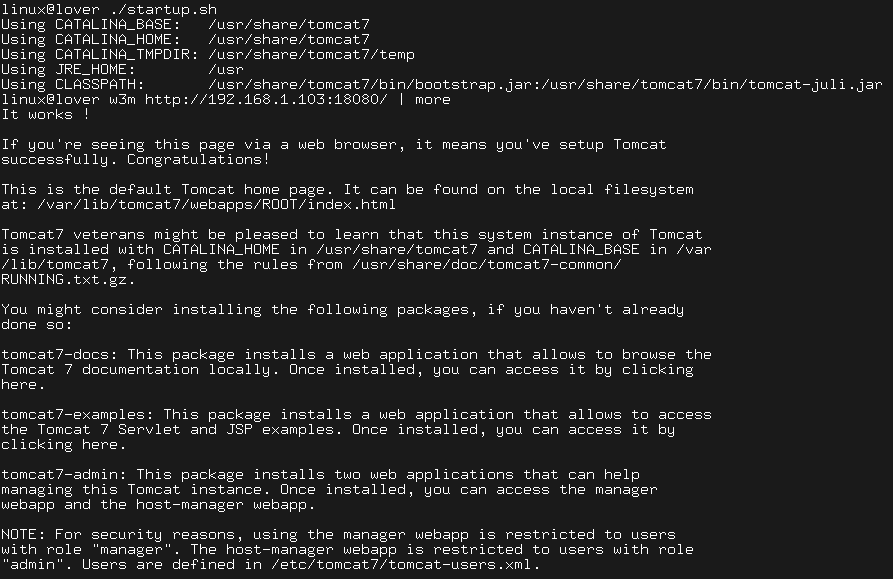
\includegraphics[width=15cm]{Success_TC.png}
			\caption{Inicialización del servicio Tomcat y comprobación de su correcto funcionamiento.}
			\label{fig:TC_Success}
		\end{figure}

		Para facilitar estos pasos y poder iniciar, apagar y reiniciar el servicio desde cualquier
		parte sin necesidad de introducir la dirección a los script cada vez que los queramos usar,
		podemos valernos de \textit{alias}.
		
		Por ejemplo, \textit{TCstart} para llamar a \textit{startup.sh}, \textit{TCstop} para llamar
		a \textit{shutdown.sh} y \textit{TCrestart} para ejecutar \textit{TCstop \&\& TCstart}.
	
\section{WildFly}
	En la página oficial de JBoss\cite{WF_official}, se nos describe como un servidor de aplicaciones
	implementado en Java en código abierto y desarrollado por \textbf{Redhat} bajo la licencia
	\textit{GNU Lesser General Public License(LGPL)}, version 2.1.
	
	Comenzó en manos de Marc Fleury, otro empleado de \textit{Sun Microsystems} y posteriormente fue
	comprada por la compañía \textbf{RedHat}.

	Posteriormente, JBoss fue renombrado por votación popular\cite{WF_vote}\cite{WF_install} y su nuevo
	nombre(\textit{WildFly}) fue anunciado en la conferencia Devoxx 2013.\cite{WF_install}\cite{WF_name}

	\subsection{Instalación y control básico del servicio(\textit{start, stop y restart})}
		Para realizar la instalación del WildFly, nos basamos en las instrucciones detalladas
		en \cite{WF_install}.
		
		Tras haber descargado el archivo adecuado de \cite{WF_download}, descomprimimos el archivo
		en la carpeta deseada.
		
		Ahora, para inciar el servicio, bastaría con ejecutar el script \textit{standalone.sh}
		o el script \textit{domain.sh}.
		
		La instalación se realiza de una manera correcta pero al intentar ejecutar el servicio,
		se produce una serie de errores(como podemos ver en la figura \ref{fig:WF_Fail}) que nos
		impiden dar comienzo al servicio\footnote{Como se detalla en \cite{WF_install}, hay otro
		modo para inicializar el servicio, ejecutando \textit{domain.sh} pero igualmente genera
		una serie de errores similares a la ejecución de \textit{standalone.sh}}.

		\begin{figure}[h!]
			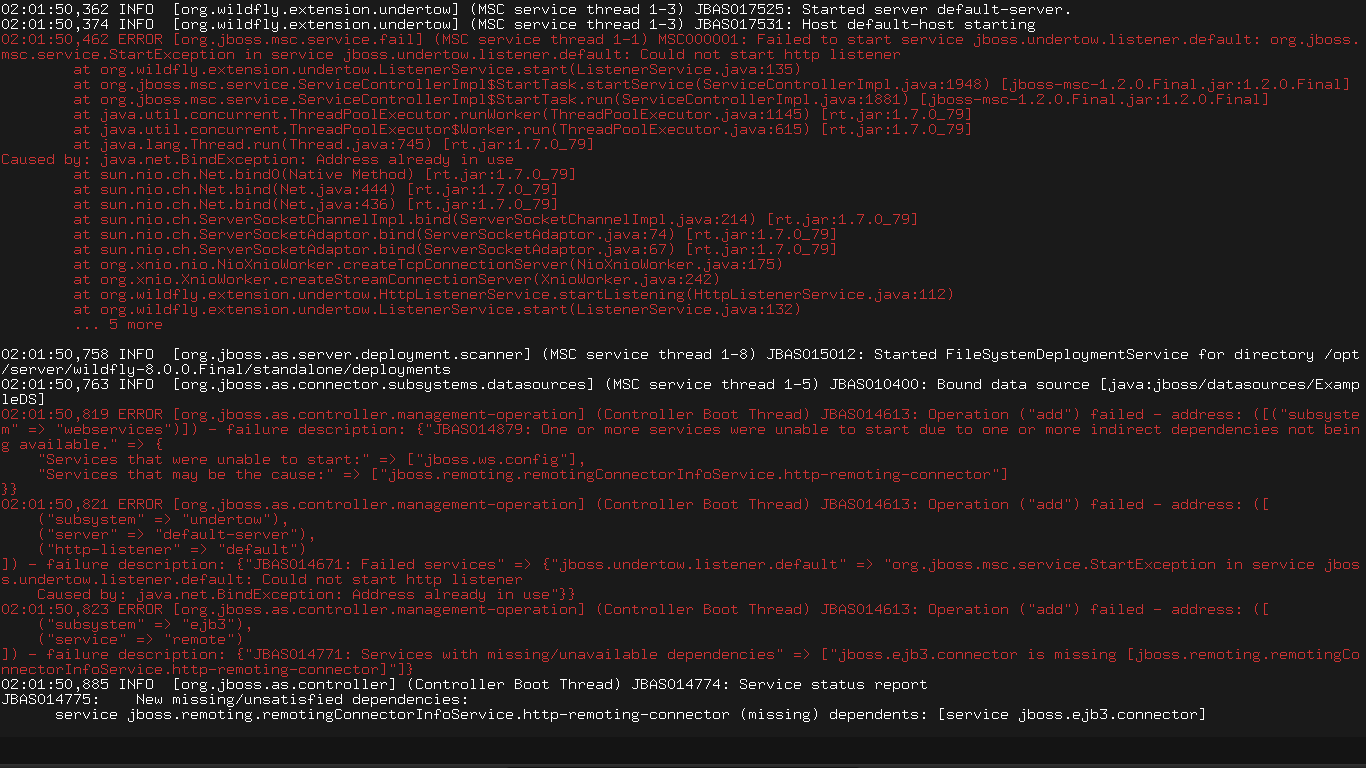
\includegraphics[width=15cm]{Fail_WF.png}
			\caption{Error al iniciar el servicio de WildFly.}
			\label{fig:WF_Fail}
		\end{figure}

		Suponiendo que hubiésemos solucionado este error, una vez seguido las instrucciones de
		\cite{WF_install}, para iniciar o apagar el servicio, disponemos de \textit{service
		wildfly start} para iniciar y \textit{service wildfly stop} para apagarlo(a diferencia
		de Tomcat, para el cuál tuvimos que crear los alias).

\section{GlassFish}

	Al igual que WildFly, GlassFish es un servidor de aplicaciones implementado en Java en código
	abierto y desarrollado por \textbf{Oracle Corporation} bajo una licencia dual \textit{Common
	Development and Distribution License (CDDL) \& GNU General Public License (GPL)} con una ligera
	modificación.\cite{GF_official}\cite{GF_install}
	
	En sus orígenes, fue desarrollado por \textit{Sun Microsystems} y posteriormente esta compañía
	fue adquirida por \textbf{Oracle Corporation}, por lo que el programa pasó a manos de los
	desarrolladores de Oracle.

	\subsection{Instalación y control básico del servicio(\textit{start, stop y restart})}
		Para realizar la instalación del servicio, nos basamos en las instrucciones detalladas
		en \cite{GF_install}.
		
		Una vez descargado el archivo comprimido de \cite{GF_download}, selecionamos la carpeta
		donde queremos ubicar el programa y lo descomprimimos.
		
		Acabada la instalación, basta con dar comienzo con el comando asadmin a un dominio para
		empezar a funcionar(análogamente, se procedería para apagar el servicio).
		
		En este proceso, la instalación se realizó de forma exitosa pero como podemos ver en la
		figura \ref{fig:GF_Fail}, cuando intentamos dar comienzo al servicio, nos produce un
		error que no he logrado subsanar haciendo, por tanto, imposible la comparativa de los
		servicios.

		\begin{figure}[h!]
			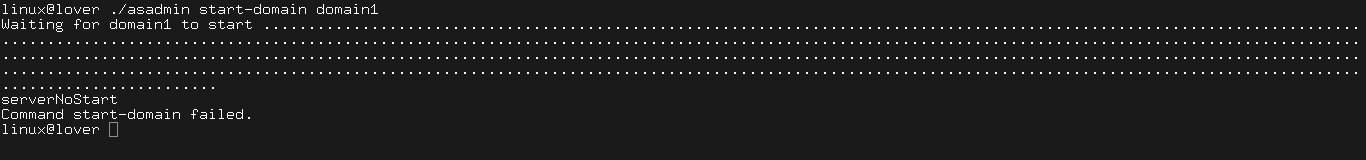
\includegraphics[width=15cm]{Fail_GF.png}
			\caption{Error al iniciar el servicio de GlassFish.}
			\label{fig:GF_Fail}
		\end{figure}

		Suponiendo que hubiésemos solucionado este error, en GlassFish usaremos el comando
		\textit{asadmin} con los parámetros \textit{start-domain}, \textit{stop-domain} o
		\textit{restart-domain} seguidos del nombre de algún dominio creado previamente
		para iniciarlo, pararlo o reiniciarlo, respectivamente.

\section{Comparación de resultados}
	La realización de esta comparativa está inspirada en las tesis de:
		\begin{itemize}
			\item John Jairo Mendez Romero\cite{JJMR_Tesis}, de la cuál tomé el código de
			ejecución en los servidores de aplicaciones.
			
			\item Diego Paul Tamayo Barriga\cite{DPTB_Tesis}, de ella surgió la idea de utilizar
			las herramientas de benchmarking: \textit{ab} y \textit{sar}. Aunque él no llega a
			utilizar el comando \textit{ab} pero sí lo presenta y da una referencia que me
			permitió investigarlo y utilizarlo.
		\end{itemize}

	Para realizar la medición de resultados de los diferentes servidores de aplicaciones(de haber
	sido posible su instalación de manera exitosa), se iba a utilizar 4 máquinas virtuales para
	interpretar los roles de cliente y cada uno de los servidores.
	
	En cada máquina servidor, se configura la aplicación correspondiente de entre nuestras 3 
	candidatas: Tomcat, WildFly y GlassFish. Una vez configuradas con algún código de ejecución
	simple, se procede a pausar dos de las máquinas servidoras para que no afecten a la ejecución
	y medición de la tercera.
	
	Desde la máquina cliente, hacemos una petición al servidor web activo haciendo uso del comando
	\textit{ab} del paquete \textit{apache2-utils} que, tal como se nos indica en su página
	oficial\cite{AB_official}, es una herramienta de benchmarking de servidores HTTP. Como podemos
	 ver en la misma página, le podemos pasar una serie de parámetros a dicho comando.
	
	Para esta prueba, se utilizarán los parámetros:
	\begin{itemize}
		\item \textit{-b} que ajusta el tamaño del buffer de envío/recepción TCP. Le daremos un rango
		de valores variando entre 1 y 100(En concreto, se usarán 1, 10 y 100).
		\item \textit{-c} que determina cuántas peticiones se pueden lanzar a la vez. Para este parámetro,
		usaremos los valores 1(por defecto), 2 y 5.
		\item \textit{-n} que determina cuántas peticiones al servidor se realizarán. En este proyecto,
		le daremos los valores 10, 50 y 100.
	\end{itemize}
	
	Esto supone un total de 27 ejecuciones por cada servidor, haciendo un total de 81.
	
	Tras cada ejecución del comando \textit{ab} con sus correspondientes parámetros, se ejecutarán
	en la máquina virtual servidor sobre la que se ha ejecutado otro comando de benchmarking llamado
	\textit{sar} del paquete \textit{sysstat}.
	
	Dicho comando permite una serie de comandos que nos
	permiten conocer diferentes aspectos sobre los que usar benchmarking, como podemos ver en su página
	oficial\cite{SAR_official}.
	
	Para esta prueba, se utilizarán los parámetros:
	\begin{itemize}
		\item \textit{-r} que muestra el estado de utilización de la memoria RAM.
		\item \textit{-u} que muestra el estado de utilización de la CPU.
	\end{itemize}
	
	Después, realizaríamos un estudio de los datos del cuál se sacaría qué aplicación nos produce
	una productividad más rápida a menor consumo de CPU y RAM. También podríamos ver qué aplicación
	es más adecuada para un servidor que dé más importancia a la CPU que a la RAM o viceversa.

\section{Perspectivas futuras}
	Para futuros trabajos, se podría comparar dichos servidores de aplicaciones con otras herramientas
	de las usadas en este documento para compararlos. Así como realizar la comparativa entre otro
	conjunto de servidores de aplicaciones de J2EE.
	
	También se podría optar por comparar varios servidores de aplicaciones con mayor heterogeneidad,
	esto es, con distinta plataforma de soporte, distinto lenguaje de programación o, incluso,
	comparar aplicaciones comerciales frente a las de libre distribución.
	
	Si tomamos un número significativo de servidores de aplicaciones de distintas plataformas,
	podríamos realizar una comparativo no sólo a nivel individual de servidores de aplicaciones, si
	no a nivel más general, comparando así las plataformas sobre las que se desarrollan.
	

\newpage
\begin{thebibliography}{10}
	\expandafter\ifx\csname url\endcsname\relax
	  \def\url#1{\texttt{#1}}\fi
	\expandafter\ifx\csname urlprefix\endcsname\relax\def\urlprefix{URL }\fi
	\expandafter\ifx\csname href\endcsname\relax
	  \def\href#1#2{#2} \def\path#1{#1}\fi
	
	\bibitem{J2EE_Def}
	\textbf{Java Platform, Enterprise Edition.} Wikipedia, the free encyclopedia.\\
		\url{https://en.wikipedia.org/wiki/Java_Platform,_Enterprise_Edition}
	
	\bibitem{API_Def}
	\textbf{Application Programming Interface.} Wikipedia, the free encyclopedia.\\
		\url{https://en.wikipedia.org/wiki/Application_programming_interface}
	
	\bibitem{RMI_Def}
	\textbf{Java Remote Method Invocation.} Wikipedia, the free encyclopedia.\\
		\url{https://en.wikipedia.org/wiki/Java_remote_method_invocation}
	
	\bibitem{JMS_Def}
	\textbf{Java Message Service.} Wikipedia, the free encyclopedia.\\
		\url{https://en.wikipedia.org/wiki/Java_Message_Service}
	
	\bibitem{Servlet_Def}
	\textbf{ORACLE Help Center.}\\
		\url{http://docs.oracle.com/javaee/6/api/javax/servlet/Servlet.html}
	
	\bibitem{JSP_Def}
	\textbf{JavaServer Pages.} Wikipedia, the free encyclopedia.\\
		\url{https://en.wikipedia.org/wiki/JavaServer_Pages}
	
	\bibitem{BL_Def}
	\textbf{Business Logic.} Wikipedia, the free encyclopedia.\\
		\url{https://en.wikipedia.org/wiki/Business_logic}

	\bibitem{AS_Def}
	\textbf{Application Server.} Wikipedia, the free encyclopedia.\\
		\url{https://en.wikipedia.org/wiki/Application_server}

	\bibitem{WS_Def}
	\textbf{Web Service.} Wikipedia, the free encyclopedia.\\
		\url{https://en.wikipedia.org/wiki/Web_service}
	
	\bibitem{TC_official}
	\textbf{Apache Tomcat}\\
		\url{http://tomcat.apache.org/}

	\bibitem{TC_TomEE}
	\textbf{Apache TomEE}\\
		\url{http://tomee.apache.org/apache-tomee.html}

	\bibitem{TC_OpenJPA}
	\textbf{Apache Tomcat}\\
		\url{http://openjpa.apache.org/}

	\bibitem{TC_MyFaces}
	\textbf{Apache MyFaces}\\
		\url{http://myfaces.apache.org/}

	\bibitem{TC_install}
	\textbf{\textit{Apache Tomcat 7 Essentials}}\\
	Tanuj Khare\\
	Ed. Packt Publishing (March 2012)\\
	Sec. "1. Installation of Tomcat7"\\
		\url{http://proquest.safaribooksonline.com/book/operating-systems-and-server-administration/apache/9781849516624}
	
	\bibitem{TC_download}
	\textbf{Apache Tomcat}\\
		\url{http://tomcat.apache.org/download-70.cgi}

	\bibitem{TC_config}
	\textbf{\textit{Tomcat The Definitive Guide}}\\
	Jason Bittain \& Ian F. Darwin\\
	Ed. O'Reilly Media, Inc. (June 2003)\\
	Sec. "1. Getting Started with Tomcat"\\
		\url{http://proquest.safaribooksonline.com/book/programming/java/0596003188}
	
	\bibitem{WF_official}
	\textbf{JBossDeveloper}\\
		\url{http://jbossas.jboss.org/}\\
		\url{http://wildfly.org/}
	
	\bibitem{WF_vote}
	\textbf{JBossDeveloper}\\
		\url{http://jbossas.jboss.org/rename/vote}
	
	\bibitem{WF_install}
	\textbf{\textit{WildFly: New Features}}\\
	Filippe Costa Spolti\\
	Ed. Packt Publishing (May 2014)\\
	Sec. "1. Starting with WildFly"\\
		\url{http://proquest.safaribooksonline.com/9781783285891?uicode=goliat} 

	\bibitem{WF_name}
	\textbf{Slideshare.net}\\
	Dimitris Andreadis-Senior Engineering Manager, JBoss EAP / WildFly at Red Hat.\\
		\url{http://es.slideshare.net/dandreadis/2013-11devoxxwild-flybof}

	\bibitem{WF_download}
	\textbf{JBossDeveloper}\\
		\url{http://wildfly.org/downloads/}
	
	\bibitem{GF_official}
	\textbf{GlassFish}\\
		\url{https://glassfish.java.net/}

	\bibitem{GF_install}
	\textbf{\textit{Java EE 7 with GlassFish 4 Application Server}}\\
	David R. Heffelfinger\\
	Ed. Packt Publishing (March 2014)\\
	Sec. "1. Getting Started with GlassFish"\\
		\url{http://proquest.safaribooksonline.com/book/programming/java/9781782176886}
		
	\bibitem{GF_download}
	\textbf{GlassFish}\\
		\url{https://glassfish.java.net/download.html}
	
	\bibitem{JJMR_Tesis}
	\textbf{\textit{Análisis comparativo de las plataformas J2EE y .NET aplicado
	al desarrollo de servicios web}}\\
	John Jairo Mendez Romero\\
	Universidad de Pamplona-Colombia(Nov. 2008)\\
		\url{http://www.j2ee-vs-net.blogspot.com.es/}
	
	\bibitem{DPTB_Tesis}
	\textbf{\textit{Análisis comparativo de los servidores GlassFish y JBoss para
	la plataforma JavaEE aplicado al módulo de catálogos del sistema de Recursos
	Humanos de la ESPOCH}}\\
	Diego Paul Tamayo Barriga\\
	Escuela Superior Politécnica de Chimborazo-Ecuador(2014)\\
		\url{http://dspace.espoch.edu.ec/bitstream/123456789/3328/1/18T00551.pdf}

	\bibitem{AB_official}
	\textbf{Apache Docs}\\
		\url{http://httpd.apache.org/docs/2.2/programs/ab.html}
	
	
	\bibitem{SAR_official}
	\textbf{Welcome to the SYSSTAT Utilities Home Page!}\\
		\url{http://sebastien.godard.pagesperso-orange.fr/man_sar.html}
\end{thebibliography}

\end{document}
